\chapter{Kết quả}
\label{Chapter5}

\textit{Nội dung chương này sẽ trình bày về các kết quả mà nhóm đã đạt được trong quá trình giải quyết các bài toán con để hoàn thành đồ án.}

\section{Kết quả của quy trình thu thập dữ liệu}
Sau khi thực hiện xong việc Scraping data, kết quả thu được là \textbf{232321} cặp câu hỏi và câu trả lời, có ngày tháng được hỏi ở hai định dạng dữ liệu là CSV và JSON.

Dữ liệu ban đầu thu thập về là ở định dạng file CSV nhưng vì lý do cần phải xử lý định dạng lại cấu trúc hiển thị dữ liệu trên website nên nhóm đã chuyển đổi định dạng của file CSV sang file JSON. 

Qua đó, nhóm đã giải quyết xong được bài toán đầu tiên cần phải giải quyết trong các bàn toán nhỏ cần phải giải để có hoàn thành được hệ thống.

\section{Kết quả sau khi mã hoá dữ liệu câu hỏi sau khi thu thập và lưu vào Elasticsearch}
Sau khi thêm dữ liệu thành công vào trong Elastic Search, để kiểm tra thông tin lưu trong Elastic Search thì ta thực hiện mở URL sau trên trình duyệt:

\begin{lstlisting}
	http://localhost:9200/demo_simcsejson/_search?pretty=true
\end{lstlisting}

Sau khi truy cập vào URL trên, Elastic Search sẽ trả về dữ liệu được lưu trữ trong có dạng như sau:

\begin{figure*}[htp]
\centering
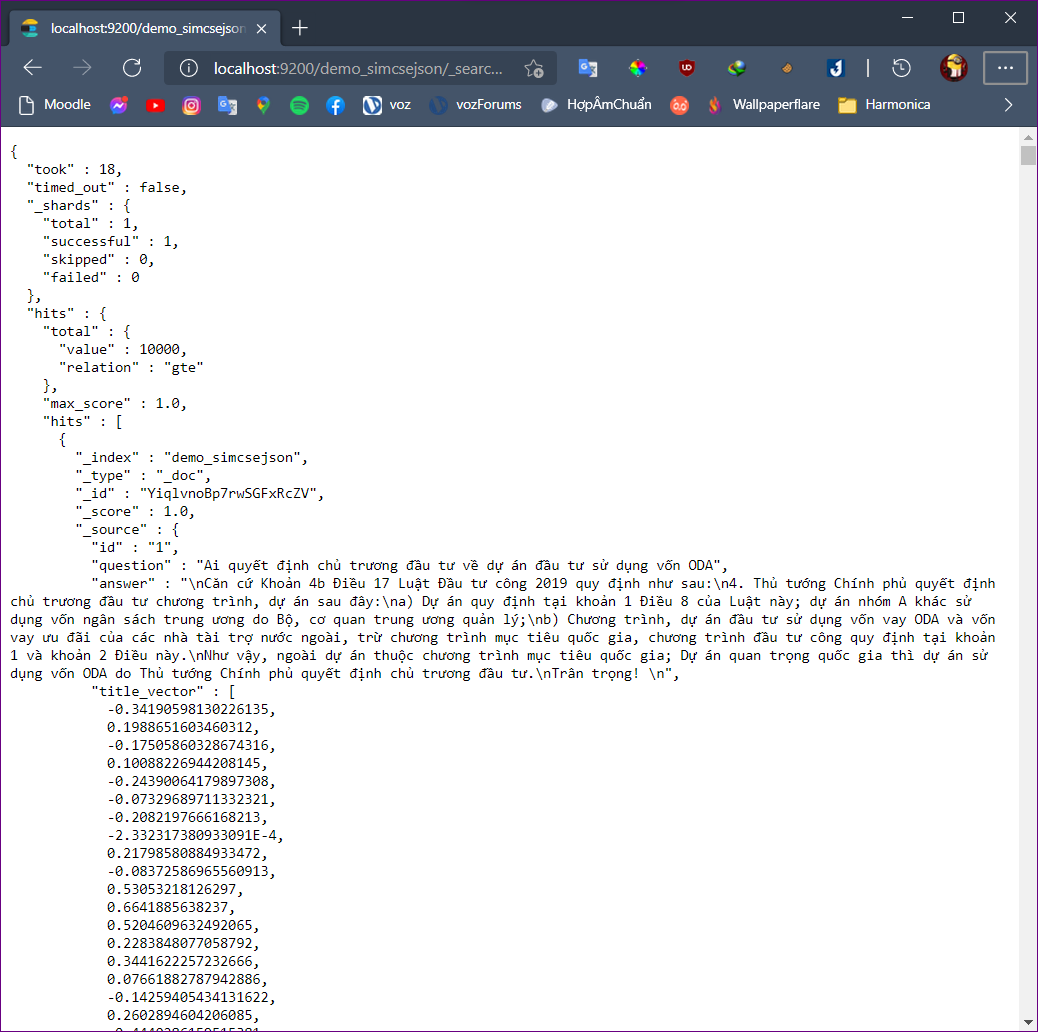
\includegraphics[width=\linewidth]{images/elastic_search_result}
\caption{Dữ liệu được lưu vào trong Elasticsearch sau khi Encode.}
\label{fig:elastic_search_result}
\end{figure*}
\pagebreak

Những mục cần lưu ý trong dữ liệu được tô đỏ trong hình ảnh trên chính là những cột dữ liệu được lưu trữ trong Elasticsearch. Những thuộc tính đã được nhấn mạnh là cần lưu trữ đã được nêu ở chương 4 là những thuộc tính nằm trong phần được đánh dấu đỏ.

Qua nội dung này thì nhóm đã hoàn thành được việc giải bài toán mã hoá văn bản tiếng việt và xử lý ngôn ngữ tự nhiên.
\section{Kết quả của quy trình nhận dữ liệu từ Back-end và hiển thị lên Front-end}

Sau khi đã lấy ra được tập câu hỏi và trả lời thoả mãn được yêu cầu của hệ thống thì cần phải trả về kết quả ra để phía web server có thể lấy được kết quả trả về để gửi lại phía bên phía Front-end, hiển thị kết quả cho người dùng.

Respond dữ liệu từ Back End lên Front End:

Template Engine: jinja2

Với việc sử dụng jinja2 là một template engine, ta có thể hiển thị dễ dàng các biến results và raw\_text đã được truyền vào trước đó bởi hàm render\_template bằng cách gọi trực tiếp trong các HTML template:

\begin{lstlisting}
	<p class="input" style="...">Cau hoi da nhap: "{{raw\_text}}"</p>
	<p class="input" style="...">{{results[0][1]}}</p>
\end{lstlisting}

Kết quả nhận được là: 
\begin{figure*}[htp]
	\centering
	
\includegraphics{images/res1}
	\caption{Kết quả của render template.}
	\label{fig:res1}
\end{figure*}

Jinja2 còn có thể dùng để viết ra các hàm để xử lý dữ liệu được đổ vào Website:

\begin{lstlisting}
	{% if results != null %}
		{{answer(answer=results[0][2])}}
		{% endif %}		
		\end{lstlisting}
		
		Kết quả nhận được là: 
		
		\begin{figure*}[htp]
			\centering
			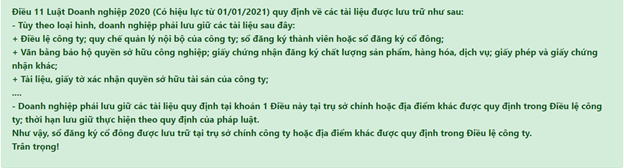
\includegraphics{images/res2}
			\caption{Kết quả nhận được khi sử dụng Jinja2.}
			\label{fig:res2}
		\end{figure*}
		
		
		\begin{lstlisting}
			{% for para in results if para[0] != 1 %}
				{{group_QA(data_id = para[0] - 1,
						question = para[1],
						answer = para[2])}}
				{% endfor %
				\end{lstlisting}
				
				Kết quả nhận được là: 
				
				\begin{figure*}[htp]
					\centering
					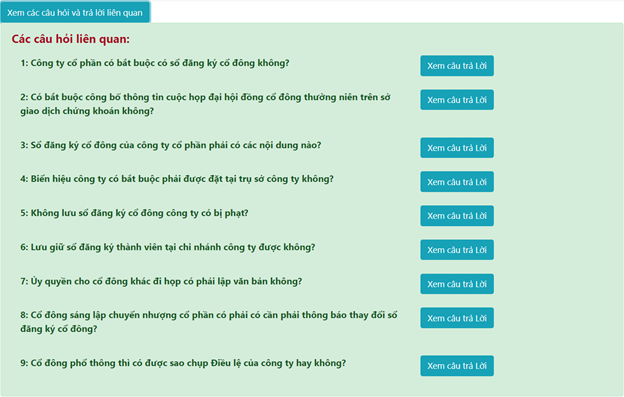
\includegraphics[scale=0.8]{images/final}
					\caption{Kết quả nhận được khi nhấn vào button "Xem câu hỏi liên quan".}
					\label{fig:final}
				\end{figure*}
\section{Tính đúng đắn của mô hình sau khi đánh giá thủ công}

Cuối cùng, để đánh giá được mô hình sử dụng trong đồ án có độ chính xác là bao nhiêu, nhóm thực hiện đánh giá thủ công trên 100 câu hỏi. Đánh giá mô hình được dựa trên so sánh độ chính xác của kết quả trả về đầu tiên (là kết quả được trả về với độ chính xác cao nhất từ hệ thống) của 3 phương pháp là:
\begin{itemize}
	\item [-] Phương pháp tìm kiếm bằng từ khoá của Elasticsearch.
	\item [-] Phương pháp tìm kiếm bằng mô hình áp dụng Pre-trained SimCSE.
	\item [-] Phương pháp tìm kiếm bằng mô hình sử dụng Pre-trained SimCSE và được sắp xếp lại bằng mô hình tự xây dựng trên dữ liệu STS và dữ liệu Pháp luật gán nhãn thủ công.
\end{itemize}

Kết quả trả về của từng phương pháp được tính như sau:
\begin{itemize}
	\item Phương pháp tìm kiếm bằng từ khoá của Elasticsearch: Kết quả được trả về là kết quả có \textit{\_score} cao nhất. Công thức tính được \textit{\_score} được Elasticsearch giải thích là:
	\begin{center}
	$IDF score * TF score * fieldNorms$\\
	\end{center}

	Trong đó, TF score là tần suất xuất hiện của term trong field. Càng xuất hiện nhiều, relevance càng cao. Term frequency (tf) của t trong document d được tính bằng căn bậc hai của số lần t xuất hiện trong d. Vậy nên ta sẽ có công thức để tính TF score là: $tf(t, d) = \sqrt{frequency}$\\
	IDF score là đánh giá tần suất xuất hiện của term trên toàn bộ index, càng xuất hiện nhiều, càng ít thích hợp. IDF score được tính theo công thức là: $idf(t) = 1 + \log{\frac{numDocs} {docFreq+1}}$\\
	fieldNorms là đánh giá độ dài của field. Field càng ngắn, thì term sẽ có giá trị càng cao; và ngược lại. fieldNorms sẽ được tính theo công thức là: $norm(d) =\frac{1}{\sqrt{numTerms}}$\\
	Các giá trị này sẽ được Elasticsearch hỗ trợ tính toán.
	\item Phương pháp sử dụng Pre-trained SimCSE: Kết quả trả là góc nhỏ nhất giữa vector câu hỏi của người dùng và vector câu hỏi có trong cơ sở dữ liệu.
	\item Phương pháp sử dụng Pre-trained SimCSE kết hợp với mô hình xây dựng trên bộ dữ liệu STS và Pháp luật thì ngoài kết quả là góc của vector thì còn có khoảng cách Euclide giữa các vector đấy là nhỏ nhất.
\end{itemize}

Sau khi chọn ra được câu hỏi đầu tiên từ hệ thống thông qua 3 phương pháp được nêu trên, nhóm có bảng kết quả thực hiện đánh giá như sau:
\begin{itemize}
	\item L1 là khi sử dụng bằng cách tìm kiếm từ khoá sử dụng Elasticsearch 
	\item L2 là khi tìm kiếm bằng mô hình áp dụng Pre-trained SimCSE
	\item L3 là khi tìm kiếm bằng mô hình sử dụng Pre-trained SimCSE và được sắp xếp lại bằng mô hình tự xây dựng trên dữ liệu STS và dữ liệu Pháp luật gán nhãn thủ công.
	\item C1 là số lượng câu hỏi được đánh giá có liên quan đến câu hỏi đầu vào ở website hoidap.thuvienphapluat.vn.
	\item C2 là số lượng câu hỏi được đánh giá có liên quan đến câu hỏi đầu vào ở Hệ thống Hỏi đáp Pháp luật Việt Nam.
	
\end{itemize}

\pagebreak

\begin{longtable}{|>{\hspace{0pt}}m{0.038\linewidth}|>{\hspace{0pt}}m{0.531\linewidth}|>{\hspace{0pt}}m{0.038\linewidth}|>{\hspace{0pt}}m{0.038\linewidth}|>{\hspace{0pt}}m{0.038\linewidth}|>{\hspace{0pt}}m{0.04\linewidth}|>{\hspace{0pt}}m{0.042\linewidth}|}
	\caption{Bảng rút gọn 100 câu hỏi dùng để kiểm tra độ chính xác của model}\\ 
	\hline
	\textbf{ID} & \textbf{Question} & \textbf{L1} & \textbf{L2} & \textbf{L3} & \textbf{C1} & \textbf{C2} \endfirsthead 
	\hline
	1 & Bán hàng rong có phải đăng ký kinh doanh không ? & 1 & 1 & 1 & 1 & 8 \\ 
	\hline
	2 & Điều kiện hưởng lương hưu của sĩ quan, quân nhân & 1 & 1 & 1 & 1 & 6 \\ 
	\hline
	3 & Thời hạn sang tên sổ đỏ khi mua bán đất & 0 & 0 & 1 & 2 & 10 \\ 
	\hline
	4 & Điều kiện mang thai hộ vì mục đích nhân đạo & 0 & 1 & 1 & 8 & 10 \\ 
	\hline
	5 & Có được khai sinh là ngày âm lịch không? & 0 & 0 & 0 & 2 & 1 \\ 
	\hline
	6 & Lương và chế độ việc làm của phụ nữ trong thời gian nuôi con nhỏ? & 0 & 1 & 0 & 0 & 8 \\ 
	\hline
	7 & Mức phạt bán buôn thuốc lá không rõ nguồn gốc xuất xứ? & 0 & 1 & 1 & 1 & 10 \\ 
	\hline
	8 & Không lập biên bản có được tạm giữ xe không? & 1 & 1 & 1 & 2 & 9 \\ 
	\hline
	9 & Mức phạt khi vi phạm về sử dụng lao động chưa thành niên & 0 & 1 & 0 & 0 & 7 \\ 
	\hline
	10 & Bảo đảm dự thầu áp dụng trong trường hợp nào? & 1 & 1 & 1 & 2 & 8 \\ 
	\hline
	11 & Quy trình đấu thầu lại sau khi hủy thầu như thế nào? & 0 & 0 & 0 & 0 & 5 \\ 
	\hline
	12 & Thời gian nộp, thời gian hoàn trả bảo đảm thực hiện hợp đồng & 0 & 0 & 0 & 2 & 6 \\ 
	\hline
	13 & Hỏi về thời điểm đóng thầu & 0 & 0 & 0 & 0 & 5 \\ 
	\hline
	14 & Có được bổ sung nhà thầu liên danh? & 0 & 1 & 1 & 1 & 6 \\ 
	\hline
	15 & So sánh đầu tư trực tiếp nước ngoài và đầu tư gián tiếp nước ngoài & 0 & 0 & 0 & 1 & 9 \\ 
	\hline
	16 & Thủ tục chuyển nhượng dự án đầu tư cho nhà đầu tư nước ngoài & 1 & 1 & 1 & 7 & 7 \\ 
	\hline
	17 & Thành lập chi nhánh công ty có vốn đầu tư nước ngoài cần làm gì? & 0 & 0 & 1 & 4 & 5 \\ 
	\hline
	18 & Độ tuổi được lập di chúc?~ & 0 & 1 & 1 & 1 & 7 \\ 
	\hline
	19 & Dưới 18 tuổi có được phép lập di chúc không? & 1 & 1 & 0 & 0 & 10 \\ 
	\hline
	20 & Nếu có nhiều di chúc ở nhiều thời điểm khác nhau, di chúc nào có hiệu lực? & 1 & 1 & 1 & 4 & 7 \\ 
	\hline
	21 & Các trường hợp nào cháu được hưởng di sản thừa kế của ông bà? & 0 & 1 & 1 & 2 & 10 \\ 
	\hline
	22 & Con riêng có được hưởng thừa kế? & 1 & 1 & 1 & 6 & 10 \\ 
	\hline
	23 & Không thực hiện nghĩa vụ phụng dưỡng cha mẹ có được hưởng thừa kế? & 1 & 1 & 1 & 0 & 2 \\ 
	\hline
	24 & Tiền phúng viếng là tài sản của ai? & 0 & 0 & 1 & 0 & 8 \\ 
	\hline
	25 & Người đã chết có được hưởng di sản thừa kế không? & 0 & 1 & 1 & 0 & 8 \\ 
	\hline
	26 & Quy định về phân chia di sản thừa kế theo pháp luật mới nhất & 1 & 0 & 1 & 2 & 9 \\ 
	\hline
	27 & Điều kiện có hiệu lực của di chúc bằng miệng? & 1 & 1 & 1 & 3 & 9 \\ 
	\hline
	28 & Chưa có giấy chứng nhận quyền sử dụng đất chia thừa kế được không? & 0 & 1 & 1 & 0 & 8 \\ 
	\hline
	29 & Đánh bạc nhiều lần bị phạt thế nào? & 0 & 0 & 0 & 2 & 10 \\ 
	\hline
	30 & Xử phạt khi sử dụng ma túy lần đầu? & 0 & 1 & 0 & 0 & 5 \\
	\hline
\end{longtable}

\pagebreak

Qua bảng kết quả đánh giá trên thì nhóm có công thức để đánh giá kết quả tìm kiếm bằng 3 phương pháp trên là:

\begin{center}
	$result = \frac{\sum_{t=1}^{N}(L_{i}(1))}{N}$    
\end{center}

Với 
\begin{itemize}
	\item \textbf{$\sum_{t=1}^{N}(L_{i}(1))$} là tổng số các giá trị bằng 1 có trong bảng đánh giá của cột kết quả đánh giá L1, L2, L3
	\item \textbf{N} là tổng số câu hỏi được đem ra làm mẫu để đánh giá các phương pháp, ở đây N có giá trị là 100.
\end{itemize}

\begin{center}
	$result' = \frac{\sum_{t=1}^{N}(C_{i}(1))}{N*10}$    
\end{center}
\begin{itemize}
	\item $C_{i}$  là số lượng câu hỏi được đánh giá có liên quan đến câu hỏi đầu vào.
	\item $N$ là tổng số câu hỏi được test, $N$=100.
	
\end{itemize}
Kết quả trả về đầu tiên mà hệ thống trả về sẽ được các thành viên đánh giá thủ công. Kết quả nào được thành viên kiểm thử đánh giá là đúng so với câu hỏi người dùng thì sẽ có giá trị là \textbf{1} và ngược lại.

\begin{itemize}
	\item Phương pháp tìm kiếm bằng Elasticsearch: 43\%
	\item Phương pháp tìm kiếm bằng mô hình Pre-trained SimCSE: 74\%
	\item Phương pháp tìm kiếm bằng mô hình Pre-trained SimCSE kết hợp với mô hình xây dựng trên dữ liệu Luật pháp: 49\%
	\item Hệ thống website hoidap.thuvienphapluat.vn: 8.2\% 
	\item Hệ thống Hỏi đáp Pháp luật Việt Nam: 74\% 
	
\end{itemize}

Qua kết quả đánh giá, mặc dù Elasticsearch rất có danh tiếng trong khả năng tìm kiếm dữ liệu với độ chính xác cao và nhanh chóng, nhưng khi áp dụng trí tuệ nhân tạo vào trong bài toán tìm kiếm thì độ chính xác của việc tìm kiếm đã được cải thiện tới 31\%. Bên cạnh đó, việc đào tạo trên dữ liệu Pháp luật với khối lượng dữ liệu Pháp luật nhỏ(chỉ 400 dòng dữ liệu) đã có cải thiện hơn 6\% so với khi chỉ sử dụng tìm kiếm bằng từ khoá thông thường. Vậy nên, nếu như mô hình được đào tạo và xây dựng lại với khối lượng dữ liệu nhiều hơn thì việc nâng cao độ chính xác của mô hình lên là việc chắc chắn sẽ xảy ra. 